\documentclass{journal}[IEEEtran, twocolumn]             % No modificar

% PASO 1. Reemplace "Práctica 1" por el número de la práctica que corresponda
\newcommand{\dochead}{Práctica 2}     

% PASO 2. Reemplace "TÍTULO PRÁCTICA" por el título de la práctica que corresponda.
\newcommand{\docsubhead}{PSD de señales aleatorias}  

% PASO 3. Reemplace "B1A - 02" por el grupo de la asignatura y el número de su grupo de laboratorio
\newcommand{\teamname}{C1}     

% PASO 4. OPCIONAL: Reemplace "\docsubhead \docsubhead" por el título del documento en caso de requerirse.
\newcommand{\titulo}{\dochead: \docsubhead}      

% PASO 5. Reemplace "31 de diciembre de 2030" por la fecha de su documento
\newcommand{\fecha}{8 de septiembre de 2024}      

% To load packages
\usepackage[T1]{fontenc}
\usepackage[utf8]{inputenc} 
\usepackage[spanish]{babel}
\usepackage[letter,left=2.0cm,top=2.0cm,right=2.0cm,bottom=4.0cm]{geometry}
\usepackage{amsmath}
\usepackage{amsfonts}
\usepackage{fancyhdr}
\usepackage{fancyvrb}
\usepackage{listings}
\usepackage{array}
\usepackage{graphicx,color,enumerate}	
\usepackage{multirow} 
\usepackage{multicol}
\usepackage{authblk}
\usepackage{charter}    % Font typeface
\usepackage{titling}
\usepackage{url}
\usepackage{hyperref}
\usepackage{xcolor}
\usepackage{booktabs}

\definecolor{uisgreen}{RGB}{125,194,3}
\definecolor{gray97}{gray}{.97}
\definecolor{gray75}{gray}{.75}
\definecolor{gray45}{gray}{.45}

\setlength{\droptitle}{-1.8cm}
\pagestyle{fancy}

%%% Header definition
\headheight=60pt 						% header height 
\renewcommand{\headrulewidth}{4pt}
\let\oldheadrule\headrule% Copy \headrule into \oldheadrule
\renewcommand{\headrule}{\color{uisgreen}\oldheadrule}

\fancyhead[L]							% left header 
{	\begin{minipage}{2.5cm}
		
\includegraphics[scale=0.3]{./figs/uislogohoriz.png} 
	\end{minipage}	
	\begin{minipage}{5cm}
	    \color{uisgreen}
	    \footnotesize {\textsf{Universidad Industrial de Santander\\ 
				Escuela de Ingenierías Eléctrica, \\
				Electrónica y de Telecomunicaciones	}}	
	\end{minipage}
}
\fancyhead[R] { 							%la "C" indica al centro
	\begin{minipage}{8cm}
	    \color{uisgreen}
	    \begin{flushright}
    	    \small{\textsf{Laboratorio de COMUNICACIONES I (27139)}} \\
            \normalsize{\textsf{\dochead: \textbf{\docsubhead}}} \\
    	    \small{\textsf{Grupo: \textbf{\teamname}}}
	    \end{flushright}
    \end{minipage}
    \begin{minipage}{1.2cm}
		
\includegraphics[width=1.0\textwidth]{./figs/logoE3T.png} 
	\end{minipage}	
}
%%% End header definition

\lstset{ frame=Ltb,
     framerule=0pt,
     aboveskip=0.5cm,
     framextopmargin=3pt,
     framexbottommargin=3pt,
     framexleftmargin=0.4cm,
     framesep=0pt,
     rulesep=.4pt,
     backgroundcolor=\color{gray97},
     rulesepcolor=\color{black},
     %
     stringstyle=\ttfamily\color{red!50!brown},
     showstringspaces = false,
     basicstyle=\small\ttfamily,
     commentstyle=\color{gray45},
     keywordstyle=\color{blue}\bfseries,
     %
     numbers=left,
     numbersep=15pt,
     numberstyle=\tiny,
     numberfirstline = false,
     breaklines=true,
   }

% minimizar fragmentado de listados
\lstnewenvironment{listing}[1][]
   {\lstset{#1}\pagebreak[0]}{\pagebreak[0]}

\lstdefinestyle{consola}
   {basicstyle=\scriptsize\bf\ttfamily,
    backgroundcolor=\color{gray75},
   }

\lstdefinestyle{C}
   {language=C,}             % No modificar


\begin{document}                    % No modificar

\title{\textbf{\titulo}}            % No modificar

% PASO 6. Agregar aquí el nombre y código de los autores.  
\author{
Sergio Camilo Santos - 2172315\\
Brayan Julian Niño Hurtado - 2172301\\
Carlos Alberto Cetina - 2215583\\
\href{https://github.com/scsantosdth/CommunicationsII_2024_2_scb.git}{https://github.com/scsantosdth/CommunicationsII_2024_2_scb.git}
}

\affil{\small{Escuela de Ingenierías Eléctrica, Electrónica y de Telecomunicaciones} \\ % No modificar
\small{Universidad Industrial de Santander}} % No modificar

\date{\fecha}                       % No modificar

\maketitle                          % No modificar
\thispagestyle{fancy}               % No modificar

%---------------------------------------------------------------
% PASO 7. **..**...****INICIE SU DOCUMENTO DESDE AQUI***...**...
%%%%% A PARTIR DE AQUÍ EDITE EL DOCUMENTO PARA AGREGAR TODO EL CONTENIDO REQUERIDO PARA EL ENTREGABLE CORRESPONDIENTE
%%%%  Todo el contenido a partir de este punto es SOLAMENTE ILUSTRATIVO.
%
% Para sus imformes, BORRE TODO el contenido de aquí en adelante  EXCEPTO la última línea que contiene el comando: \end{document}


\color{black}

\begin{multicols}{2}

\begin{abstract}
    Este informe presenta el análisis y cálculo de la Densidad Espectral de Potencia (PSD) de señales aleatorias utilizando GNURadio como herramienta principal. Se emplearon tanto bloques propios de GNURadio como funciones personalizadas para generar señales y calcular su PSD. El objetivo principal es comprender la estructura espectral de las señales y su energía distribuida en función de la frecuencia, interiorizando conceptos clave sobre señales aleatorias y el cálculo de promedios.

 \textit{\textbf{Palabras clave: Densidad Espectral de Potencia, señales aleatorias, GNURadio, PSD, promedios, análisis espectral.}} 
\end{abstract}

\section{Introducción}
   En este laboratorio, se estudiará el uso de herramientas y funciones de GNURadio para calcular la PSD de señales aleatorias. Implementando no solo bloques ya disponibles en la plataforma, sino que también funciones personalizadas para generar y analizar señales, comprendiendo mejor los conceptos de señales aleatorias y el análisis espectral.


\section{Metodología}
\subsection{Parte A: Comprobar el funcionamiento del frujograma}
Se implementó el flujograma propuesto analizando el comportamiento de una señal binaria aleatoria bipolar de forma rectangular. Se observó su forma, su forma en el tiempo, además de calcular su Densidad Espectral de Potencia (PSD). Se obtuvo la frecuencia de muestreo, ancho de banda y rata de bits, para diferentes valores de Sps (Samples per symbol) ajustando el valor de la variable h la cual define el tamaño del vector.



\subsection{Parte B: Comprobar como es el ruido blanco}
Para comprobar el ruido blanco en tiempo y en PSD, se configuraron dos bloques 'Virtual Source'  denominados p4 y p5. Se generó ruido blanco utilizando un bloque 'Noise Source'  y se realizaron varias priuebas ajustando la amplitud. 

 
\subsection{Parte C: Análisis de señal de una imagen}
En esta parte, se evaluó el comportamiento de la señal cuando los bits provienen de una fuente del mundo real. Para ello, se modificó el flujograma reemplazando el bloque "Random Source" por los bloques "File Source" y "Unpack K Bits", permitiendo la lectura del archivo "rana.jpg" y la extracción de sus bits. Posteriormente, se realizaron varias pruebas para observar la representación de la señal en el dominio temporal y su Densidad Espectral de Potencia (PSD). Este análisis permitió visualizar cómo se comporta la señal en comparación con una fuente aleatoria, basándose en las gráficas obtenidas.

\subsection{Parte D: Análisis de señal de un micrófono}
Se estudió el comportamiento de la señal en los dominios temporal y frecuencial utilizando datos de audio provenientes de un micrófono. Para ello, se configuró el bloque "File Source" para leer el archivo "sonido.wav", lo que permitió capturar los bits que representan la grabación. A través de gráficas generadas, se registraron observaciones y conclusiones que resaltan las diferencias en la estructura de la señal y su comportamiento espectral, en especial la Densidad Espectral de Potencia (PSD), en comparación con fuentes de datos más aleatorias.

\subsection{Parte E: Preguntas de control}
Preguntas de auto control sobre el flujograma randombinayrectsignal.grc
    
\section{Resultados}
\subsection{Parte A: Comprobar el funcionamiento del frujograma}

Como resultado, se logró visualizar la representación temporal y la Densidad Espectral de Potencia (PSD) de una señal binaria bipolar aleatoria (Figura 1). Lo que permitió examinar su comportamiento, validando los parametros con las siguientes relaciones.

    \begin{center}
    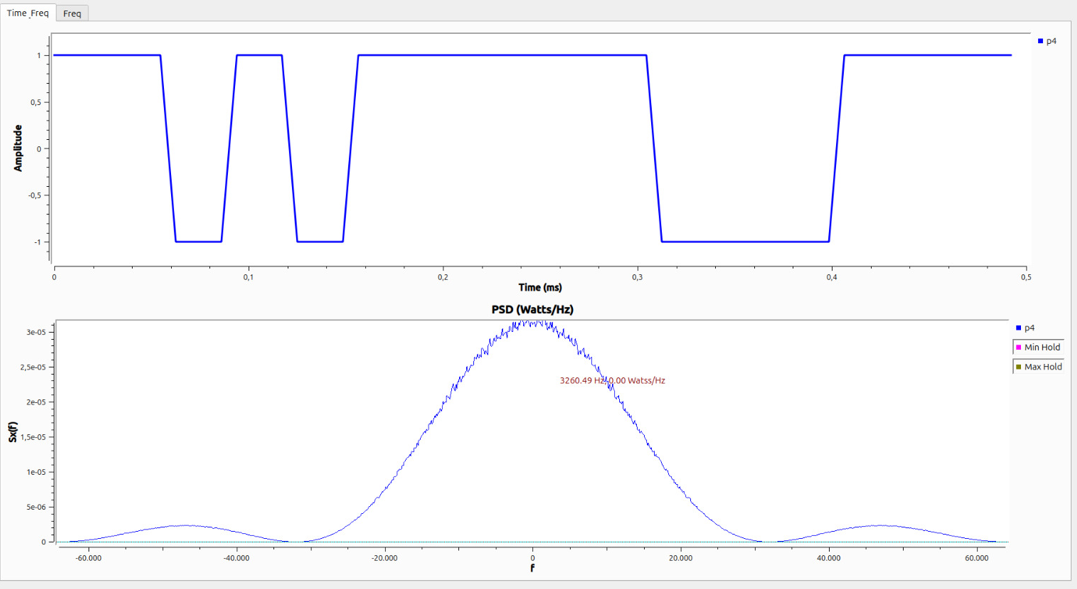
\includegraphics[width=0.45\textwidth]{figs/F1.png}
    \caption{Figura 1: Resultao gráfica en tiempo y frec (Sps=4)}
    \end{center}
    
El bit rate ($R_b$) y la frecuencia de muestreo ($f_s$) están relacionados mediante la fórmula $R_b = \frac{F_s}{sps}$.

El ancho de banda ($B$) necesario para la transmisión de la señal se puede estimar utilizando el criterio de Nyquist, que se expresa como $B = \frac{R_b}{2}$ [1].

    \begin{center}
    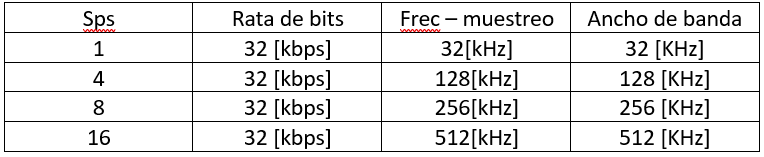
\includegraphics[width=0.45\textwidth]{figs/F2.png}
    \caption{Tabla 1: Resultado flujograma}
    \end{center}
    
Con los resultados obtenidos (Tabla 1), se observó que al incrementar el número de muestras por símbolo (Sps), también aumenta la frecuencia de muestreo ($f_s$). Este aumento se debe porque al incrementar el Sps, se mejora la resolución temporal de la señal, dividiendo cada símbolo en más muestras. Esto requiere una mayor frecuencia de muestreo para capturar con precisión los detalles de cada símbolo y representar la señal adecuadamente sin pérdida de información. 

Sin embargo, el bit rate (Rb) se mantiene constante porque, aunque aumente el número de muestras que describen un símbolo, esto no cambia la cantidad de símbolos que se envían en un segundo. ya que la frecuencia muestreo ($f_s$) crece para representar más muestras por símbolo.


\subsection{Parte B: Comprobar como es el ruido blanco}

    \begin{center}
    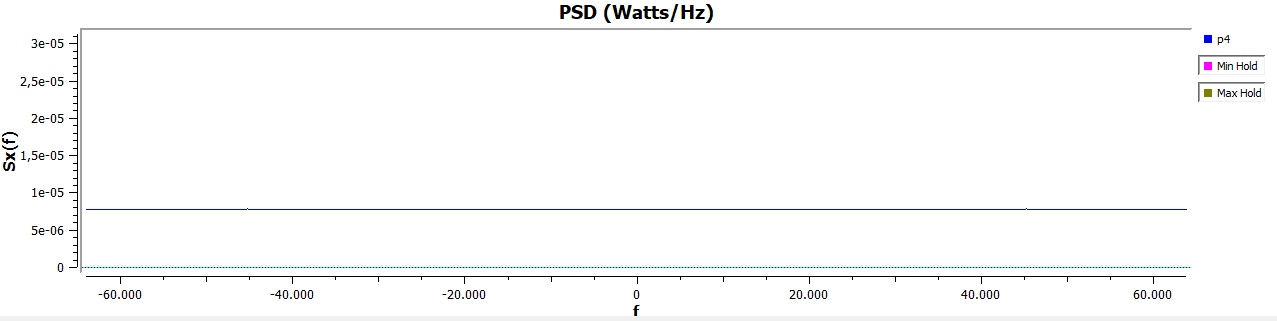
\includegraphics[width=0.45\textwidth]{figs/F3.png}
    \caption{Figura 2: PSD del ruido blanco}
    \end{center}

En los resultados obtenidos, se observó que al aumentar la amplitud del bloque "Noise Source", la Densidad Espectral de Potencia ($S_x(f)$) también crece de manera proporcional. Este comportamiento ocurre porque al incrementar la amplitud de la señal, aumenta la energía total contenida en ella, lo que se traduce en un incremento de la potencia. El aumento de potencia genera un incremento de la ganancia, directamente relacionado con la temperatura equivalente del ruido en el receptor. Dado que la Densidad Espectral de Potencia está definida por $N_0/2$, donde $N_0 = k \cdot T_e$ (siendo $T_e$ la temperatura equivalente y $k$ la constante de Boltzmann), al aumentar la temperatura, el valor de $N_0$ se incrementa. Esto explica por qué a mayor amplitud, mayor es la temperatura, la potencia y, por lo tanto, el valor de $S_x(f)$. Además, la gráfica de $S_x(f)$ constante a lo largo de todas las frecuencias confirma la naturaleza del ruido blanco, caracterizado por un espectro de potencia uniforme y un ancho de banda teóricamente infinito.


\subsection{Parte C: Análisis de señal de imagen}

    \begin{center}
    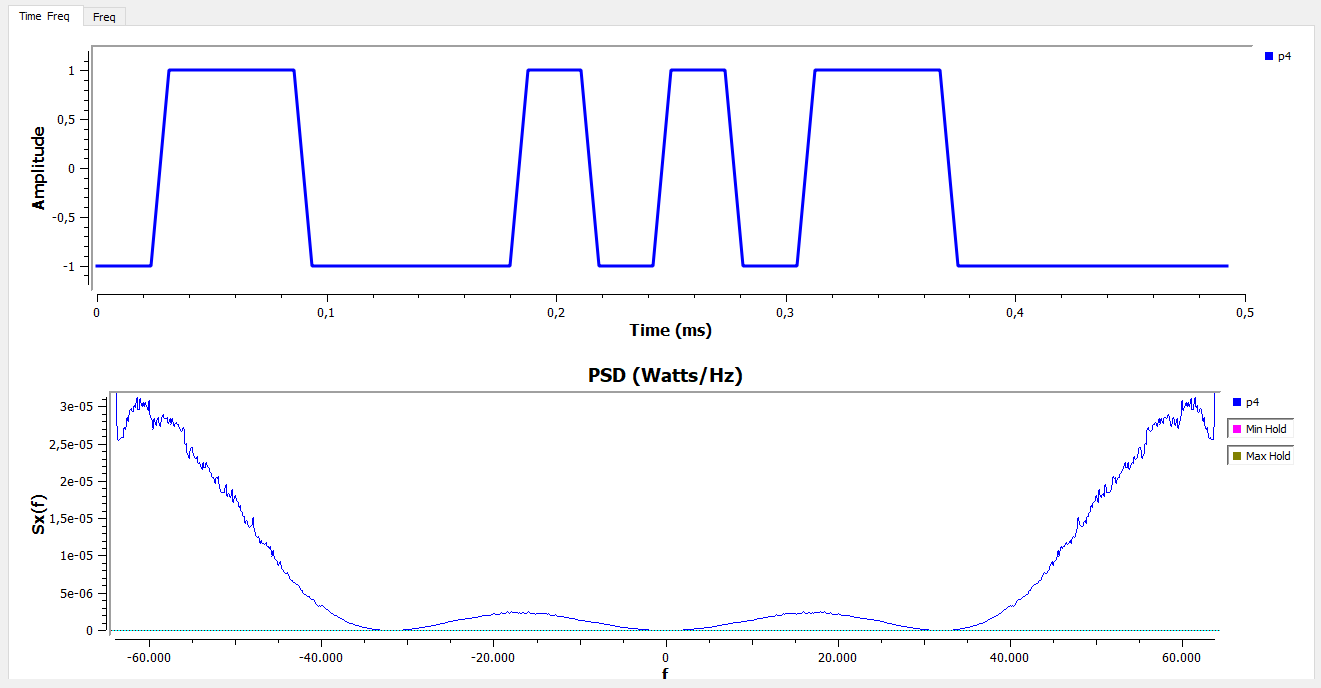
\includegraphics[width=0.45\textwidth]{figs/F4.png}
    \caption{Figura 3: Gráficas de tiempo y PSD señal de imagen}
    \end{center}


Como resultado, para las señales, cuando la fuente es una imagen, se obtuvieron gráficas similares a las de una señal binaria aleatoria bipolar, lo que se atribuye al proceso de codificación de datos. Al transformar una imagen en datos binarios, se genera una secuencia de bits que puede parecer aleatoria, especialmente en imágenes con variaciones de intensidad. Esto resulta en patrones de 0s y 1s que carecen de una estructura clara en el dominio temporal, similar a las señales binarias aleatorias. Asimismo, la Densidad Espectral de Potencia (PSD) de estas señales es comparable, ya que ambas comparten la naturaleza binaria de los datos. La conversión a bits distribuye la energía en el espectro de manera uniforme, produciendo una PSD que muestra un comportamiento similar, independientemente de la fuente de los datos.


\subsection{Parte D: Análisis de señal de un micrófono}


    \begin{center}
    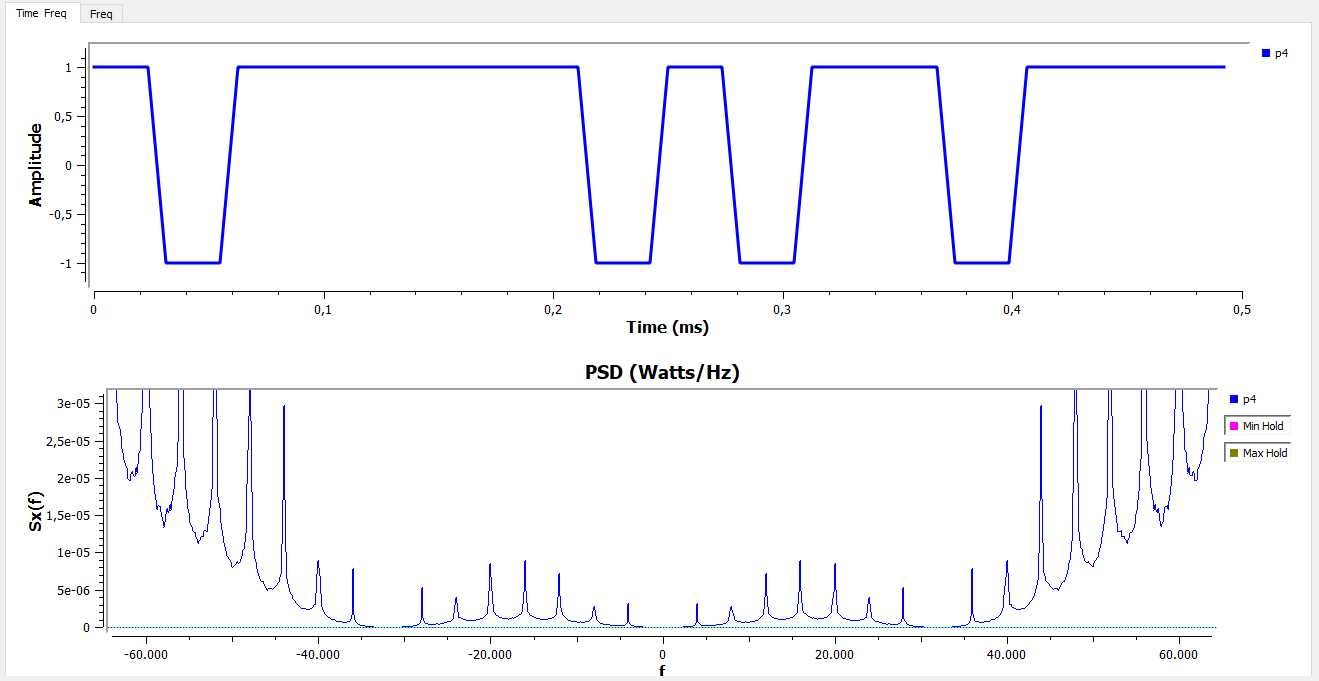
\includegraphics[width=0.45\textwidth]{figs/F5.png}
    \caption{Figura 4: Gráficas de tiempo y PSD señal de sonido}
    \end{center}
    
Al analizar la señal proveniente del micrófono, representada en el archivo de audio "sonido.wav", se observó que en el dominio temporal la señal no mostró diferencias significativas en comparación con una señal binaria aleatoria bipolar. Esto sugiere que la conversión del audio a bits binarios genera un patrón de 0s y 1s que puede parecer similar a una secuencia aleatoria, ya que en la representación temporal no se destaca la estructura del contenido del sonido. Sin embargo, en el dominio frecuencial, la Densidad Espectral de Potencia (PSD) reveló diferencias notables. Se observó una serie de pulsos o picos a lo largo del espectro, y el número de estos picos correspondía directamente con el número de bits configurados en el bloque "Unpack k bits". Esto sucede porque, al aumentar el número de bits en la descomposición de la señal, se incrementa el nivel de detalle en la representación binaria, lo que resulta en una mayor cantidad de transiciones de 0s y 1s, que se reflejan en la PSD como picos adicionales. Estos picos indican un incremento en la cantidad de información codificada por cada transición de bits, lo cual afecta la resolución y estructura espectral.

  
\subsection{Parte E: Preguntas de control}




\section{Conclusiones}

\begin{itemize}
    
    \item Se pudo validar representación de la PSD de una señal binaria bipolar aleatoria y el análisis de sus parámetros utilizando el flujograma propuesto. El aumento del número de muestras por símbolo ($Sps$) permitió observar cómo la frecuencia de muestreo se ajusta para capturar con mayor detalle cada símbolo, sin afectar el bit rate ni el ancho de banda. Asegurando que la señal se represente con precisión.
    
     
\end{itemize}

\begin{thebibliography}{1}

\bibitem{comu} 
Stanford University - Lectures on Digital Communications, \textit{https://web.stanford.edu/class/ee179/lectures/notes14.pdf}

\bibitem{wiki} 
Creating Your First Block:  \textit{https://wiki.
gnuradio.org/index.php?title=Creating_Your_First_Block}

\end{thebibliography}

\end{multicols}

\end{document}
